\section{Convolutional Neural Network}

Convolutional Neural Networks are a specialized type of Deep Learning architecture designed to automatically and efficiently extract spatial features from images.
A typical Convolutional Neural Network architecture consists of convolutional layers, activation layers, and pooling layers, which are stacked in sequence to learn increasingly abstract representations of the input data.
As the network depth increases, the number of channels (i.e., the depth of the feature maps) grows, while the spatial dimensions (height and width) of the feature maps decrease.
\begin{figure}[H]
    \centering
    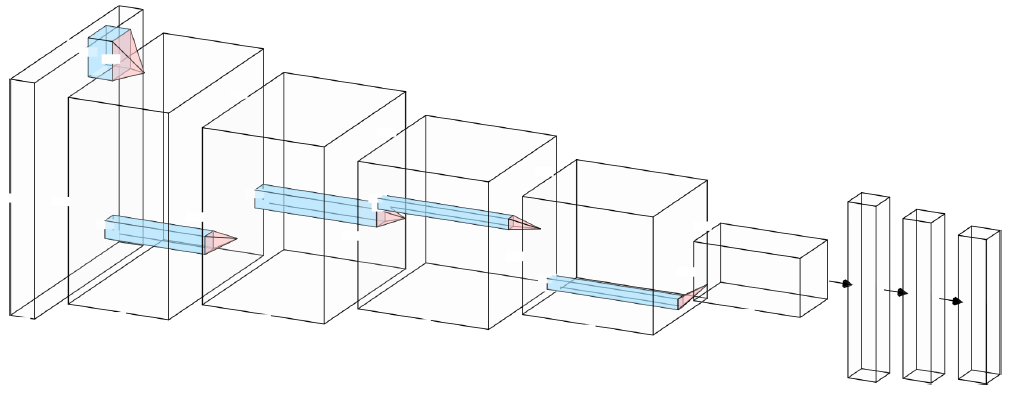
\includegraphics[width=1\linewidth]{images/cnn.png}
    \caption{Convolutional Neural Network transformations}
\end{figure}

\subsection{Convolutional layer}
The convolution operation is at the heart of a Convolutional Neural Network. 
During the convolutional layer, small regions of the input (called receptive fields) are processed using filters, which are learned during training.

The input image is represented as a volume with dimensions: height $h$, width $w$, and depth. 
The filters, which also have a defined height and width, slide over the input image to extract features at different locations. 
For each region of the input, the filter produces an output known as an activation map.

For a given filter $w$ applied over the input image, the output at a specific location $(r, c)$ and channel $l$ is computed as:
\[a(r,c,l)=\sum_{u,v,k}\mathbf{w}^l(u,v,k)x(r+u,c+v,k)+b^l\]
Here, $U$ represents the small receptive field, $C$ is the number of input channels, and $b^l$ is the bias term. 
The result of applying each filter to the input is an activation map corresponding to a particular feature.

The total number of parameters in a convolutional layer is determined by the size of the filters and the number of filters:
\[\text{parameters}=(h_r\cdot h_c\cdot c)n_f+n_f\]
Here, $h_r$ and $h_c$ are the filter's height and width, $c$  is the input depth (number of channels), and $n_f$ is the number of filters.

Key characteristics of the convolutional layers include:
\begin{itemize}
    \item \textit{Local processing}: convolutions operate over small spatial regions $U$, meaning each filter processes localized sections of the image at a time.
    \item \textit{Channel-wise processing}: filters span the entire depth of the input volume, allowing them to capture information across all channels
    \item \textit{Output volume}: each filter produces a slice of the output volume, also known as an activation map, where each filter outputs a different slice corresponding to a distinct feature.
\end{itemize}
As the input passes through successive convolutional layers, its representation becomes increasingly abstract. 
The early layers may learn simple features like edges and textures, while deeper layers capture higher-level structures like shapes and objects. 

\subsection{Activation layer}
Activation layers are crucial for introducing nonlinearities into the network, enabling Convolutional Neural Networks to model complex patterns and relationships in data.
Without these nonlinear activation functions, a Convolutional Neural Network would behave similarly to a linear classifier, severely limiting its ability to capture the intricate, hierarchical features typically present in image data.

Activation functions are applied element-wise, meaning they operate independently on each individual value in the feature map (or volume). 
While they do not alter the spatial dimensions of the feature map, they modify the values within it, enabling the network to learn more complex and abstract features.

The most widely used activation functions in Convolutional Neural Networks are ReLU and Leaky ReLU. 
These functions are preferred due to their simplicity, computational efficiency, and strong performance in deep networks. 
Both functions help mitigate issues like vanishing gradients, allowing networks to train more effectively.

\subsection{Pooling layer}
Pooling layers are designed to reduce the spatial dimensions (height and width) of the input volume while retaining the most significant features. 
This downsampling process enhances the computational efficiency of the network and helps prevent overfitting by reducing the number of parameters and computations. 
Pooling layers operate independently on each channel of the input volume, meaning they are applied separately to the depth of the feature maps.

\paragraph*{Max pooling}
The most common pooling technique is max pooling, where the maximum value is selected from a defined region (typically a square or rectangular window) of the input. 
Max pooling effectively reduces the spatial size of the input while preserving the most prominent features.

\paragraph*{Strides}
The stride determines how much the pooling window moves across the input volume during the pooling operation. 
It defines the step size between each operation as the window slides over the feature map.

In most cases, the stride is equal to the size of the pooling window, meaning the window moves non-overlapping across the input. 
However, a stride of one (unitary stride) means the pooling window moves by just one pixel at a time, creating an overlap between the regions being pooled.
This can help in extracting more detailed features without significantly reducing the spatial dimensions.

\paragraph*{Global Average Pooling}
Global Average Pooling reduces the entire feature map for each channel into one average value. 
This significantly reduces the number of parameters compared to traditional Fully Connected layers, making the network simpler and less prone to overfitting, while maintaining its ability to capture important features across the image.

Global Average Pooling is then followed by a simple softmax layer for classification. 
Thus, the number of feature maps before the Global Average Pooling layer should match the number of output classes. 
However, if there is a mismatch, a hidden layer can adjust the feature dimension.

\subsection{Architecture}
In a Convolutional Neural Network, once the spatial dimensions of the feature maps have been sufficiently reduced through successive convolutional, activation, and pooling layers, the output is flattened into a one-dimensional vector.
This vector is then fed into a traditional Fully Connected Neural Network.
At this stage, the spatial structure of the image is no longer preserved, and the network shifts focus to combining the high-level, abstract features learned in the earlier layers.

The final Fully Connected layer typically has an output size corresponding to the number of target classes, producing a score (or probability) for each class. 
The raw output scores are usually passed through a softmax activation function, which converts them into probabilities that sum to one, indicating the likelihood of each class.

Throughout the Convolutional Neural Network, convolutional filters are learned to detect patterns that are relevant to the specific classification task at hand. 
The architecture of the network generally consists of stacking multiple convolutional, activation, and pooling layers. 
\begin{figure}[H]
    \centering
    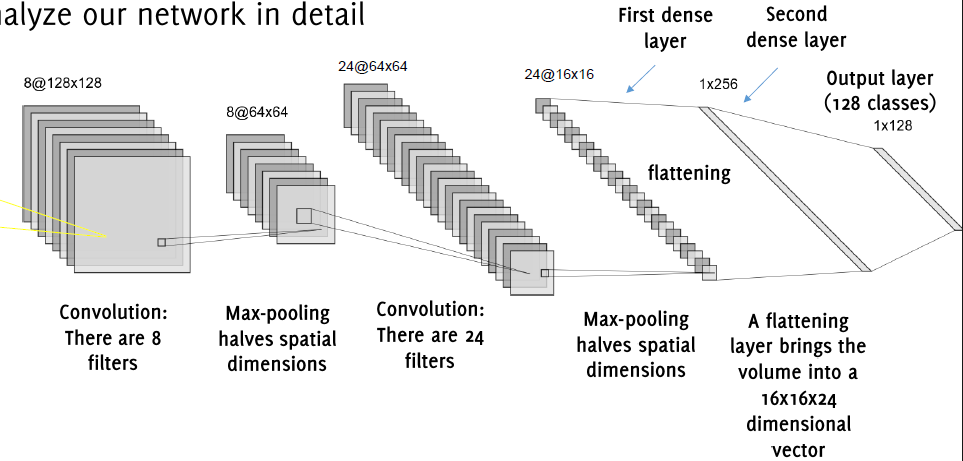
\includegraphics[width=0.75\linewidth]{images/cnn1.png}
    \caption{Convolutional Neural Network architecture}
\end{figure}

\subsection{Convolutional and dense layers}
In dense layers, the weight matrix is fully populated, meaning every neuron is connected to every other neuron in the adjacent layers. 
This leads to comprehensive interactions between neurons, allowing the network to model complex relationships. 
However, this full connectivity comes with a large number of parameters, which can make training more computationally expensive and prone to overfitting.

In contrast, convolutional layers exhibit sparse connectivity.
In these layers, each output neuron is influenced only by a subset of input neurons, which reflects the localized nature of convolutions.
As a result, most of the entries in the weight matrix are zero. 
The convolutional operation spans all channels of the input, leading to a weight matrix with a circular structure.

In convolutional layers, the weights are shared across the entire output channel. 
The same filter is applied across multiple positions of the input to compute the output. 
This means that different positions in the input share the same filter, reducing the total number of parameters in the network. 
The same filter is applied to each local region of the input, which allows the network to recognize the same feature at different spatial locations.

\paragraph*{Spatial invariance}
A defining characteristic of Convolutional Neural Networks is spatial invariance. 
This means that the network is capable of detecting features regardless of where they appear in the image.
All neurons within the same slice of a feature map use the same set of weights and biases.
This significantly reduces the number of parameters compared to Fully Connected layers, as many neurons share the same weights and biases across spatial positions.
The fundamental assumption behind this approach is that if a feature is useful in one part of the image, it should also be useful in other parts. 